\documentclass{vldb}

\usepackage[utf8]{inputenc}
\usepackage{times}
\usepackage{graphicx}
\usepackage{xcolor}
\usepackage{hyperref}
\usepackage{paralist}
\usepackage[inline]{enumitem}



\usepackage{balance}  % for  \balance command ON LAST PAGE  (only there!)

\usepackage{subcaption}
\graphicspath{{./images/}}

\newcommand{\grumbler}[2]{{\color{red}{\bf #1:} #2}}
\newcommand{\andre}[1]{\grumbler{andre}{#1}}
\newcommand{\nuno}[1]{\grumbler{nuno}{#1}}
\newcommand{\carla}[1]{\grumbler{carla}{#1}}

\newcommand{\outline}[1]{}
%\newcommand{\outline}[1]{\grumbler{outline}{#1}}

\newcommand{\emphvspace}{0.5\baselineskip}
%Single line
\newcommand{\lineemph}[1]{\vspace{\emphvspace}\hspace{2em}\emph{#1}\vspace{\emphvspace}}
%Multi line
\newcommand{\firstblockemph}[1]{\vspace{\emphvspace}\hspace{2em}\emph{#1}}
\newcommand{\middleblockemph}[1]{\hspace{2em}\emph{#1}}
\newcommand{\lastblockemph}[1]{\hspace{2em}\emph{#1}\vspace{\emphvspace}}

\vldbTitle{}
\vldbAuthors{}
\vldbVolume{12}
\vldbNumber{xxx}
\vldbYear{2020}
\vldbDOI{https://doi.org/TBD}


\begin{document}

\title{Global Views on Partially Geo-Replicated Data}
\numberofauthors{3} %  in this sample file, there are a *total*
% of EIGHT authors. SIX appear on the 'first-page' (for formatting
% reasons) and the remaining two appear in the \additionalauthors section.

\author{\alignauthor André Rijo\\
       \affaddr{NOVA LINCS, FCT, Universidade NOVA de Lisboa}\\
%       \email{v.sousa@campus.fct.unl.pt}
\alignauthor Carla Ferreira\\
       \affaddr{NOVA LINCS, FCT, Universidade NOVA de Lisboa}\\
%       \email{carla.ferreira@fct.unl.pt}
\alignauthor
Nuno Preguiça\\
       \affaddr{NOVA LINCS, FCT, Universidade NOVA de Lisboa}\\
%       \email{nuno.preguica@fct.unl.pt}
}


\maketitle

\begin{abstract}
\andre{Please review this}

Many existing web services of global scale have strict latency, availability and fault tolerance requirements.
To handle this, some services distribute their datacenters across the globe, with users accessing the closest datacenter.
As the number of servers increases, so does the replication cost, thus partial replication can be desirable.
However, some queries may require global data not replicated in every server (e.g. in an online store scenario, the top 10 most sold products globally).

In this paper, we present PotionDB, a novel geo-distributed key-value store which provides partial replication.
We present a replication scheme which allows data to be partially replicated, yet still answer queries relative to global data efficiently.
We leverage on existing partial and non-uniform replication algorithms to provide materialized views of data that may be split across multiple servers.
With these views, a client can obtain global information by querying a single server.
Our evaluation shows that queries concerning global data can be completed in less than one millisecond, while maintaining high throughput despite the extra updates required to keep the views up-to-date. 

%Geo-replicated, distributed data stores that support complex online applications, such as social networks, must provide an “always- on” experience where operations always complete with low latency. Today’s systems often sacrifice strong consistency to achieve these goals, exposing inconsistencies to their clients and necessitating complex application logic. In this paper, we identify and define a consistency model—causal consistency with convergent conflict handling, or causal+—that is the strongest achieved under these constraints.
%We present the design and implementation of COPS, a key-value store that delivers this consistency model across the wide-area. A key contribution of COPS is its scalability, which can enforce causal dependencies between keys stored across an entire cluster, rather than a single server like previous systems. The central approach in COPS is tracking and explicitly checking whether causal dependen- cies between keys are satisfied in the local cluster before exposing writes. Further, in COPS-GT, we introduce get transactions in or- der to obtain a consistent view of multiple keys without locking or blocking. Our evaluation shows that COPS completes operations in less than a millisecond, provides throughput similar to previous systems when using one server per cluster, and scales well as we increase the number of servers in each cluster. It also shows that COPS-GT provides similar latency, throughput, and scaling to COPS for common workloads.


\end{abstract}

\section{Introduction}

%	\item Num. DC a aumentar

The increasing reliance on web service in many domains of activity, from e-commerce to business applications
and entertainment, leads to stringent requirements regarding latency, availability and fault tolerance \cite{Schurman2009latency,gomez}.
To address these requirements, cloud platforms have been adding new data centers at different geographic 
locations. By allowing users to access a service by contacting the closest data center, a global service can
provide low latency to users spread across the globe. The increasing number of data centers also contributes
for proving high availability and fault tolerance, by allowing a user to access the service by accessing any
available data center.

% serviços necessitam de data
% Replicar totalmente tem problemas

The database is a key component of any web service, storing the service's data. For supporting global
services running at multiple geographic locations, it is necessary to rely on a geo-replicated database \cite{dynamo},
which maintains replicas of the data at the data centers where the service is running.
A number of geo-replicated databases have been proposed, providing different consistency semantics.
Databases that provide strong consistency \cite{spanner,cockroachdb,mdcc} intend to give  the illusion that 
a single replica exists, requiring coordination among
multiple replicas for executing (update) operations. This leads to high latency and may compromise 
availability in the presence of network partitions.
Databases that provide weak consistency \cite{eventual,dynamo,cops} allow any replica to process a
client request, leading to lower latency and high availability. As a consequence, these databases expose
temporary state divergence to clients, making it more difficult to program a system. 

In either case, geo-replicated databases typically rely on a full replication model, where each data 
center replicates the full database, with data being sharded across multiple partitions in each data 
center. 
As both the data managed by these systems increases in size and the number of data centers increases,
this approach leads to a number of problems.
First, storing all data in all data centers imposes a large overhead in terms of storage. 
Furthermore, storing some data in all data centers may be unnecessary, as data is only needed at some
geographic locations.
Second, increasing the number of data centers makes the replication process more complex and costly, 
as each update needs to be propagated to all other data centers.

For addressing these problems, partial replication is an attractive approach, with each data center
replicating only a subset of the data. A number of works have been addressing the challenges of 
partial replication, for example by proposing algorithms to manage partially replicated data \cite{more,saturn,c3}
and to decide which data is replicated in which replica \cite{}.

In this paper we address the problem of querying data in a weakly consistent partially geo-replicated database, 
focusing on recurrent queries for which a programmer would want to generate a (materialized) view.
For example, consider an e-commerce system with users from multiple geographic locations.
In this case, the data pertaining users of a given location does not need to be replicated in all data centers
(but only in a few for fault tolerance). The same applies to other information, such as data on orders and 
warehouses.
Other data, such as information on products would be replicated in the regions where the product
is available.  
Under this data placement, obtaining the list of best seller products is challenging, as it requires
accessing data that is located at multiple data centers.

Several possible solutions exist for this problem. 
First, it is possible to have a data center that replicates all data, and forward these queries to such data center.
Doing this imposes a latency penalty and requires a data center to host all data and execute all queries of this type. %Andre: also refer that this data center would be the bottleneck of the system?
Second, it is possible to execute the query by accessing multiple locations, by using, for example, 
a distributed processing system with support for geo-partitioned data %\cite{Kloudas:2015:POD:2850578.2850582,more}.
\cite{kloudas2015pixida,more}.
This approach requires running an additional external service and poses challenges for the consistency of the results
returned and the data observed by users.
%, mostly when adopting weak consistency models (a local update that should
%be reflected in the result of the query may not be returned, as the update might have not been read by the 
%external service that accessed a different replica).

We propose a different approach: to maintain materialized views, as commonly available in relational databases.
Implementing such feature efficiently in a partially geo-replicated database requires 
addressing two main challenges. 
First, it is necessary to guarantee consistency between the base data available in a replica and the 
relevant materialized views. To achieve this, we designed a replication mechanism where updates 
to the base data and views are made visible atomically in each replica.

Second, it is necessary to efficiently support views with limits, used for example to support \emph{top-k} 
queries. To achieve this, we build on the concept of non-uniform replication \cite{Cabrita17Nonuniform}, in which the state
of different replicas may be different, given that the observable state is (eventually) the same.
This allows each replica to propagate only the updates that might be relevant to the observable 
state. Providing support for views required us to extend non-uniform replication from simple data 
types to more complex structures that could support a view with multiple columns.
\nuno{can we support updates to the views? why not?}
\andre{short-answer: no. Since views don't have all data (e.g: only the name of a customer), we can't translate an update in a view to updates in other CRDTs, as such update would be incomplete}

We present the design and implementation of PotionDB, a geo-replicated key-value store with support  
for partial replication and materialized views. 
PotionDB provides weak consistency, for improved latency and availability, and support for highly
available transactions \cite{hat}.  
To our knowledge, our work is the first to address the problem of maintaining materialized views
in such setting.  

We have evaluated our system using micro-benchmarks and TPC-H queries \cite{tpch}.
The results show that our algorithms for maintaining materialized views impose 
low overhead when executing and asynchronously replicating transactions, particularly
for views with limits.
\nuno{deviamos ter uns micro-benchmarks que comparassem o overhead com limites e sem limites}
Additionally, the results show that executing queries by relying on the materialized views is much more 
efficient than using alternative mechanisms.  
Furthermore, our algorithms for maintaining materialized views in a decentralized way perform better 
that alternative approaches where the view is computed in a single data center, while being
able to  keep consistency between the base and view data in every replica.

In this paper we make the following contributions:
%\begin{enumerate*}[(label=\roman*)]
\begin{itemize}
	\item the design of a geo-replicated key-value store  with support for partial replication
	and views over partially replicated data; 
	\item replication algorithms for efficiently maintaining consistent materialized views over 
	partially replicated data;
	 \item an implementation and evaluation of the proposed approach with micro-benchmarks
	 and TPC-H.
\end{itemize}

The remainder of the paper is organized as follows. Section ...

\outline{topicos

\begin{itemize}
	\item Num. DC a aumentar
	\item Replicar totalmente tem problemas
	\item Replicação parcial
	\item Queries sobre dados replicados parcialmente
	\begin{itemize}
		\item Standard solution?
	\end{itemize}
	\item Views materializadas replicadas totalmente
	\item Contribuições
\end{itemize}
}

\section{Motivation example}
\label{sec:example}

%TODO: I need to include here the complete example query. And explain why the tradicional way with key-value stores is non-efficient. And why a view theorically makes it both easier and more efficient.
%Use as a starting point the text in "Old stuff that may still be useful"

In order to both facilitate the understanding of the rest of the paper, as well as show the usefulness of queries supported by materialized views, we present the following example scenario.

Consider a large scale commerce company with stores and clients spread across the world.
Assume the company keeps data of millions of products, with each store having its own stock of products available.
Also consider that there are millions of both current and past customers and, among other data, all sales ever done are kept in the database, for both product warranty and statistical purposes.

Fully replicating the whole dataset would have proibitive costs.
It is also unecessary, as both the relevance of the data and likehood of being accessed from are dependent on the location.
For instance, an asian customer is more likely to consult the stock of stores in his country rather than in an european country.
Thus, it makes sence that both asian customers' and asian stores' data to be replicated mainly in asian datacenters (plus possibility a subset of others for fault tolerance purposes).
That is, the servers for which data will be replicated can be choosen based on the geographic location, as its relevance depends on such factor.

To keep the example simple, we will only consider three types of objects: customers, products and sales.
The simplified scheme of each object can be found on Figure \ref{fig:objects}.

\begin{figure}
	%\begin{table}[]
	\centering
	\begin{tabular}{|l|l|}
		\multicolumn{2}{c}{Customer} \\ \hline
		id            & int          \\ \hline
		name          & string       \\ \hline
		age           & int          \\ \hline
		country       & string      \\
		\hline
	\end{tabular} \hspace{0.7em}
	\raisebox{0.225\height}{\begin{tabular}{|l|l|}
			\multicolumn{2}{c}{Products} \\ \hline
			id           & int           \\ \hline
			name         & string        \\ \hline
			value        & int   \\
			\hline       
	\end{tabular}} \hspace{0.7em}
	\begin{tabular}{|l|l|}
		\multicolumn{2}{c}{Sales} \\ \hline
		id            & int       \\ \hline
		custID        & int    \\ \hline
		productID     & int       \\ \hline
		amount        & int	\\
		\hline      
	\end{tabular}
	\caption{Example objects}
	\label{fig:objects}
	%\end{table}
\end{figure}

Customers represent clients that at some point in time have bought at least one product from one of the stores.
Products represents items that may be (or have been) for sale.
Sales represents the aquisition of one or more units of a product by a client, where custID and productID refer to, respectivelly, the customer's and product's id field.

For the purpose of this example, we'll consider the following replication scheme for each type of object:
\begin{itemize}
	\item \emph{Customer:} replicated in the data centers present in the continent correspondent to his country (plus a few other data centers for fault-tolerance purposes);
	\item \emph{Products:} replicated in all datacenters;
	\item \emph{Sales:} replicated in the same data centers as of the customer who bought the product. 
\end{itemize}

Despite the fact that some objects aren't replicated everywhere, PotionDB will still support queries that refer to a global view of the database.
E.g., queries such as ``top 100 customers who have spent the most across all stores'' must be efficiently handled by PotionDB, even though no server contains all customer and sales data. 
This kind of queries allows to gather important real-time statistics which allow businesspersons to make decisions and changes on the business strategy to improve its rentability.
\andre{Should I refer tpc-h here?}

The following is an example of a query requiring a global view of the database:

\lineemph{Get the top 100 customers who have spent the most across all stores. For each customer, the name, age, country and total value spent must be returned.}

Without views and by using just the three kinds of objects in Figure \ref{fig:objects}, executing this query would require communication with multiple datacenters across the world, as both sales and customers' data is partitioned.
Since there are millions of customers and sales records, this would imply downloading large amounts of data and also spending a considerable amount of CPU time for data joining.
After the joins are complete, it is still needed to calculate the total value spent for each customer and sort descendingly based on the total value spent by each customer.
Only after this whole process is complete can the query be answered correctly.
Due to the sheer amount of data involved, this query would have unnaceptable performance if executed in this way.

Defining the right view(s) avoids having to do for each query the process referred above.
For the example query above, a view that keeps, for each customer, his name, age, country and total value, ordered by total value, can answer efficiently the query with a single get operation.
With this we no longer need to contact multiple datacenters and execute millions of gets and result processing.

On Section \ref{subsec:viewsconsistency} we address multiple difficulties related to supporting and keeping views updated, as well as our solutions for such difficulties in PotionDB.

\section{System Overview}

PotionDB is a geo-distributed storage system which provides weak consistency or, more precisely, causal consistency.
A key feature in PotionDB is the ability to efficiently provide global views on partially replicated data under the conditions mentioned previously.
In this section we discuss design decisions which made it possible to provide such feature.

\subsection{System model}

We consider an asynchronous distributed system composed by a set of servers S connected by a network. 
We assume the network may delay, duplicate or re-order messages, but does not corrupt them. 
We also assume messages sent are eventually delivered, even if connections may temporarely drop.

Database objects are replicated in one or more servers, but not necessarely in all of them.  
We consider a server to be a replica of an object if it replicates such object. 
New updates are sent periodically to replicas asynchrnously. 
We don't require for all updates to be delivered to all replicas, as will be detailed in Sections \ref{subsubsec:replication} and \ref{subsubsec:nureplication}
%However, not all updates need to be delivered to every replica - only updates that modify the objects' visible state must be delivered eventually \ref{non-uniform}.

Clients connect to one or more servers. 
Updates and queries are executed in a single server and return as soon as its execution ends.
Clients may group multiple operations together in a single transaction.
Only objects replicated in the server may be accessed, i.e., to access objects not present in a given server, the client must connect to a replica of those objects.

\subsection{System API}

\subsubsection{Key-value store API}

PotionDB provides a key-value store interface \cite{???}.
%PotionDB is a key-value store database. %TODO: Reference?
As such, all objects are indexed by a key and support \emph{get} and \emph{update} operations which, respectively, query/modify the state of an object.
In PotionDB objects are CRDTs \cite{???}, which ensures that even if objects are modified concurrently in different replicas, their states will eventually converge.
This allows for both \emph{get} and \emph{update} operations to be executed locally, with the effects of \emph{updates} being propagated asynchronously to other replicas.

To ease development of applications that use PotionDB, both \emph{gets} and \emph{updates} may refer to either the full object state or part of it.
A \emph{get} has the following interface: %\\

%Get CRDT key bucket crdtType\{arguments\}\\
\lineemph{Get CRDT key bucket crdtType\{arguments\}}

The triple key, bucket, crdtType are mandantory arguments used to uniquely identify an object.
Bucket is used mainly for partial replication purposes, as will be described in Section \ref{subsubsec:replication}. 
Arguments are optional as they're used only if reading part of the state, with the possible arguments depending on the type of CRDT. 
E.g., for a map CRDT, we could use: 

\lineemph{Get CRDT customer1 customers MAP\{name, age\}}

%to return only the values in the customer1 map CRDT referred by the map keys name and age.
to return only the name and age of a customer stored as a map CRDT.

\emph{Updates} have a similar interface:

\lineemph{Update CRDT key bucket crdtType\{arguments\}}

Key, bucket and crdtType have the same meaning as in \emph{get}.
The type of arguments depend on the type of CRDT, and each CRDT may support multiple types of update operations. 
E.g., a map supports both addition and removal of key/value pairs.
An insertion/update of an entry in a map can be represented as: \\

\lineemph{Update CRDT customer1 customers MAP\{ADD\{name: \\"David"\}\}}

\subsubsection{API for view CRDTs}
\label{subsubsec:APIVew}

In relational databases (and even some non-relational ones, e.g., Cassandra \cite{???}) it is common to have \emph{views}. 
A view can be defined as being the result of a query on one or multiple objects \cite{???}.
Views can be acessed as if they were normal objects, thus it eases the definition of new queries.
%TODO: Does this need a SQL example here?

Views can either be materialized or not (albeit not all databases support both). %TODO: references 
In a materialized view, the result of the query is stored as an object, which can then be reused later \cite{???}.
This may potencially improve drastically the performance of certain queries, but incours an extra cost on updates, as both the object and the materialized view need to be updated.
On the other hand, non-materialized views don't have this extra cost, but they also don't usually improve the performance of queries, as their result is re-calculated on each query.

PotionDB supports materialized views.
Similarly to relational databases, defining the right materialized views allows for efficient execution of complex queries.
In the case of PotionDB, views may even refer to data that isn't replicated locally.

We extend our key-value API with SQL-like sintax in order to support views.
This can be seen as a layer on top of the key-value API which offers two operations: \emph{create table} and \emph{create view}.
This layer then converts those operations to one or more \emph{gets} and \emph{updates}.

The \emph{create table} operation has the following structure:

\firstblockemph{Create Table name As}

\lastblockemph{From (key1*, bucket1*), (key2*, bucket2), ..., (keyN*, bucketN) crdtType}
%We extend our key-value API with the \emph{create view} operation.
%The operation sintax is similar to SQL's - the data to fill the view is choosen using \emph{select} and \emph{from}
%The operation sintax is similar to SQL's:

\andre{Should the create table operation also have where? E.g., group only customers of a certain nation.}

The goal of \emph{create table} is to group together multiple CRDTs under the same name, which can then be referred to by \emph{create view}.
The \emph{from} clause specifies the objects to be grouped.
Note the use of the ``*'' symbol - it means that every value which starts with the string before ``*'' will match.
E.g., for ``customer*'', both ``customer'' and ``customer1'' match.
This serves two goals - first, to more easily include existing objects and, second, to also allow to include future objects that may be latter added which should also belong to the group.

One could argue that \emph{bucket} could be used for the purpose of grouping objects for views , but doing such would mix the management of partial replication with views.
If that were done, a system admin would have to consider both how data should be replicated and which views might be created when defining buckets.
We believe that splitting view and partial replication management is easier to be deal with.

For creating the view itself, the \emph{create view} operation is used, which has the following sintax:

\firstblockemph{Create View key bucket As}

\middleblockemph{Select table1.a, table1.b, ..., tableN.a, tableN.b, ...}

\middleblockemph{From table1, ..., tableN}

\middleblockemph{Where conditions}

\middleblockemph{Group by table1.a, ...}

\lastblockemph{Order by table1.a, ...}

All the clauses in create view have the same meanings as in SQL.
\emph{From} specifies which tables to take information from, while \emph{select} chooses which fields should populate the view. 
Note that both fields and read operations can be issued in select, which allows to use as base others objects besides maps.
\emph{Where} restricts which objects should populate the view, while \emph{group} and \emph{orderBy} are optional and serve to organize the objects in the view.

Depending on \emph{select} and the presence of \emph{group by} and \emph{order by}, different types of CRDTs may be generated by the \emph{create view} operation.
Section \ref{subsec:viewsconsistency} covers in detail which kinds of views are supported in PotionDB, along with how views are kept correct and in sync with their base data.

\andre{Should I still give here an example? Before I had here an example of a view operation that generated a TopK which answered the query in Section \ref{sec:example} with just a simple get. But now it would seem odd to include such example here imo.}

\subsubsection{[OLD]API for view CRDTs}
\label{subsubsec:OLDAPIView}

In relational databases (and even some non-relational ones, e.g., Cassandra \cite{???}) it is common to have \emph{views}. 
A view can be defined as being the result of a query on one or multiple objects \cite{???}.
Views can be acessed as if they were normal objects, thus it eases the definition of new queries.
%TODO: Does this need a SQL example here?

Views can either be materialized or not (albeit not all databases support both). %TODO: references 
In a materialized view, the result of the query is stored as an object, which can then be reused later \cite{???}.
This may potencially improve drastically the performance of certain queries, but incours an extra cost on updates, as both the object and the materialized view need to be updated.
On the other hand, non-materialized views don't have this extra cost, but they also don't usually improve the performance of queries, as their result is re-calculated on each query.

PotionDB supports materialized views.
%Just like in a relational databases defining the right indexes and materialized views ensures even complex queries may be executed efficiently.
Similarly to relational databases, defining the right materialized views allows for efficient execution of complex queries.
In the case of PotionDB, views may even refer to data that isn't replicated locally.

We extend our key-value API with the \emph{link} operation.
The idea of \emph{link} is to specify how can an object (view) be updated based on updates executed on other objects (base data).
Whenever an update is issued on the base data, PotionDB will also simultaneously update the view.

The link construct has the following structure:

\firstblockemph{Link CRDT key bucket crdtType}

\middleblockemph{From (key1*, bucket1*, crdtType1), ..., (keyN*, bucketN*, crdtTypeN)}

\middleblockemph{Where conditions}

\lastblockemph{Update updateArgs}

Similarly to \emph{get} and \emph{update}, each triple key, bucket, crdtType uniquely identifies an object.
The link operation can be split in four parts:
%In short, \emph{link} specifies the CRDT that will be a view, while \emph{from} and \emph{where} specify which CRDTs will trigger updates on the view CRDT.
%Update specifies how to update the view CRDT. 
%More precisely:

\begin{itemize}
	\item \emph{Link}: specifies which CRDT will be acting as a view, i.e., the target of  \emph{update};
	\item \emph{From}: Similarly to the \emph{from} construct in SQL, it specifies which CRDT(s) will be used to build the view;
	In other words, whenever an update happens in one of these CRDTs, an update may also be triggered in the link CRDT.
	Note that in this construct exclusively, both key and bucket may be a prefix of the keys/buckets of the CRDTs (this is represented by the '*' character).
	This allows to include objects that may not yet exist in the database but that should also be included when they get added (e.g., new customers);
	\item \emph{Where}: Similary to the \emph{where} construct in SQL, it specifies using conditions how can the CRDTs returned in \emph{from} be joined/filtered. %E.g., if we only wanted sales related to portuguese customers: where customers.MAP{country} = "Portugal" \emph{and} sales.MAP{custID} = customers.MAP{id} \emph{and} sales.MAP{productID} = products.MAP{id};
	\item \emph{Update}: Specifies the operation that, for each entry returned by \emph{from} after applying \emph{where}, will be used to update the CRDT specified in \emph{link}.
\end{itemize}

The intuition is that when \emph{link} is first executed for a view CRDT, the view is updated based on all existing objects that match the \emph{from} and \emph{where} clauses.
Afterwards, whenever a CRDT that matches \emph{from} is updated, the \emph{where} clause is executed for that CRDT only and the \emph{update} part is executed on the view.
In Section \ref{subsec:viewsconsistency} we discuss in detail different possibilities for implementing this, as well as how it is done in PotionDB. %TODO

The query presented in Section \ref{sec:example} can be answered with a single \emph{get} on the Top-K CRDT generated by the following \emph{link}:

\firstblockemph{Link CRDT topsales statistics TOPK}

\middleblockemph{From (customers*, customers, MAP), (products*, products, MAP), (sales*, sales, MAP)}

\middleblockemph{Where sales.MAP\{customerID\} = customers.MAP\{id\} \emph{and}  sales.MAP\{productID\} = products.MAP\{id\}}

\lastblockemph{Update MAP\{name: customers.MAP\{name\}, age: \\ customers.MAP\{age\}, country: customers.MAP\{country\}, spent: products.MAP\{value\} * sales.MAP\{value\}\}}

\section{Partitioning, Replication and Consistency}

%In this section we discuss three important design decisions in PotionDB:
In this section we describe important mechanisms in PotionDB: partitioning, replication and transactions.
The referred mechanisms are the basis for efficiently supporting queries on global data, while still maintaing reasonable update performance and space overhead.

\subsection{Partitions}

In PotionDB objects are partitioned both internally in a server and externally between different servers.
Both partitioning mechanisms work differently and have different goals, which we explain in this subsection.

\subsubsection{Internal partitions}

\andre{This likely needs to be better motivated/explained...}

Inside a server objects are split across multiple partitions.
Each object is assigned to one partition automatically.
The partition to which an object is assigned to is determined by computing an hash based on the object's key, bucket and type.

The idea of partitioning objects internally in a server comes from the observation that, by having data grouped in multiple ``slot'' (i.e., partitions), if different clients access objects in different partitions, then both requests can be processed concurrently by a replica without any conflict.
And if both requests are read only, then they can be processed concurrently even if some objects are present in both requests, as reads don't conflict \cite{???}.
Each partition has one thread associated, which allows PotionDB to efficiently use multi-core CPUs.

At a first glance it may seem odd to partition based on a hash with the goal of improving performance.
However, this is justified by the expected use of PotionDB - simirlarly to relational databases, the most frequent and complicated queries are expected to have, for each one, a single view that answers them directly, thus requiring only a single operation.
Due to the nature of hashing, these views are very likelly be spread across multiple partitions.
This implies that multiple queries can be executed concurrently without conflicts even in the presence of concurrent updates that only affect unrelated objects.
Our practical evaluation shows that this partitioning improves PotionDB's performance quite considerably. %TODO: This very likelly won't be included in the Practical evaluation section. I may have to run some benchmarks and report the results here.

%A possible alternative to internal partitioning and still make use of multi-core CPUs would be to use locks to control access to the same object, in order to prevent write conflicts \cite{???}.
Other possible solutions to make use of multi-core CPUs are possible, for instance:
\begin{enumerate}
	\item \label{item:locks} using locks to protect the same object from being concurrently modified \cite{???};
	\item \label{item:multiplePotion} running multiple PotionDB servers in the same computer.
\end{enumerate}

%In theory this can lead to a considerate performance improvement, as each replica can make use of their multi-core CPUs by having one thread per partition to process requests.
%Other possible solutions include: 
%\begin{enumerate*}[label=(\roman*)] 
	%\item \label{item:locks} using locks to protect the same object from being concurrently modified \cite{???};
	%\item \label{item:single} using only a single thread \cite{???}.
%\end{enumerate*}

Alternative \ref{item:locks} is difficult to implement, as it is needed to find the right level of lock granularity and when should locks be obtained/released \cite{???}. 
Special care is needed to avoid deadlocking concurrent transactions. 
There's also concerns with both fairness and overhead of obtaining locks.
Our solution does not need to lock data, thus it avoids the overhead from using locks, is easier to implement and does not have deadlocks.

As for \ref{item:multiplePotion}, this would imply more replicas running in the system, which increases both replication and storage costs.
This would also imply concurrency conflicts even in the same computer.
Finally, while this can allow more clients to be processed in the same period of time, and is quite easy to implement, it does not improve the performance of each client, as each transaction must be done in a single replica (and thread) to avoid breaking consistency. %TODO: Does this need to be explained? The idea here is that we would lose the "write follows reads/writes" property.

%As for \ref{item:single}, the solution does not take any benefict from  the multiple cores of nowadays CPUs \cite{???}. In section \ref{???}, we show that this solution has worse performance than ours, specially with read-only transactions.

\subsubsection{External partitions}

Since PotionDB is a partially replicated \cite{???} database, it is necessary to have a mechanism which allows to precisely define in which servers should an object be replicated in.

We achieve this by requiring each object to be identified not only by its key, but also by a ``bucket''.
Buckets define groups of objects that are replicated in the same group of replicas, that is, two objects with the same bucket value will be replicated in the same replicas.
For each replica, the system admin can define which buckets will be replicated in it.

To exemplify, recall the commerce example presented in Section \ref{sec:example}.
The customers can be partitioned based on their country's continent by taking the following steps: 

\begin{enumerate}
	\item Define one bucket per continent;
	\item Configure the servers so that each replica replicates the bucket of its continent + another one for fault tolerance purposes;
	\item When adding a customer to the database, specify the bucket correspondent to the customer's continent.
\end{enumerate}

%PotionDB's replication mechanism takes in consideration the bucket distribution among servers, ensuring only servers interested in a given bucket receive updates for that bucket.
It's worth noting that clients must ensure they are communicating with a server which replicates the buckets they want to operate on, since each server only replicates a subset of the buckets and doesn't forward operations to other servers.

\subsection{Replication}

%Explain the basic idea of replication (async, partial, etc). Also include NuCRDTs here.
Replication in PotionDB is asynchronous and partial.
Operations are executed localy, without needing to contact other replicas.
Periodically, new updates are propagated asynchronously to other replicas.
All objects in PotionDB are operation-based CRDTs, thus the information required to propagate an update consists in the operation type and its arguments.

\subsubsection{RabbitMQ}

PotionDB uses RabbitMQ \cite{???} for handling communication between replicas.
RabbitMQ is a message brooker which allows consumers to register the topics of messages in which they're interested.
We leverage on topics to ensure each replica only fetches the messages containing updates for objects in buckets they are replicating.

We use RabbitMQ as follows.
Each PotionDB servers runs alongside it a RabbitMQ instance.
When a replica starts, it contacts other server's RabbitMQs and subscribes to all messages whose topics match the buckets it replicates.
When a replica wants to publish new updates, it splits those updates by buckets (while keeping causality), ensuring each message only contains updates for one bucket and whose topic value is that bucket.
Those updates are then sent to the local RabbitMQ instance, which then forwards them to interested PotionDB instances.

We also use RabbitMQ to support the addition of new replicas without stopping the system.
However, such mechanism is outside of the scope of this paper and thus we don't describe it here.

\subsubsection{NuCRDTs replication}
\label{subsubsec:nureplication}

Non-uniform CRDTs \cite{???} leverage on the fact that, for certain objects, not all of the object's data is necessary to answer queries.
E.g., in a Top-K CRDT that only maintains the K elements with highest value, only those K elements must be replicated in every replica.

The key difference between eventual consistency and non-uniform eventual consistency is that, instead of requiring for the states of each object to be eventually equivalent, it requires for the \emph{observable} stables to be eventually equivalent \cite{???}.
Two states are defined as observable equivalent iff, for each possible query, the result is equivalent when executed on either states.
This allows to save both storage space and communication overhead, as not all updates in a non-uniform CRDT must be replicated to all replicas \cite{???}.

Non-uniform CRDTs are specially useful for using as materialized views, as they allow to keep summaries of data easily while also being space-efficient.
E.g., in the scenario described in Section \ref{subsubsec:APIView}, even if there's millions of customers globally, replicas don't need to keep data for all customers in order to correctly apply reads in the Top-K CRDT.

\andre{What's above, technically, isn't 100\% true: all replicas together need to keep ALL entries of the top-k due to removes being supported. Thus, an entry for all customers in the system. This WILL BE reflected in the experimental evaluation's graphics. However, no single replica needs to keep all entries (albeit, as of now, one does).}

PotionDB fully supports NuCRDTs.
Thus, when an operation is applied on a NuCRDT, the operation is only replicated to all of that CRDT's replicas iff that operation changed the visible state.
Some operations however may only have an effect later (e.g: in a top-k, an element may rise to the top after another one gets removed) \cite{???}.
Operations in that category are only replicated to all replicas when it affects the visible state.

\andre{Should I refer that those operations in the last category are/should (as they aren't as of now) be sent to a few replicas for fault-tolerance purposes?}

\subsection{Transactions}

\andre{This section quite likely still needs to be heavily worked on, but I don't know how to proceed with it...}
%Somehow explain that we'll cover casual consistency/PotionDB's consistency guarantees in the transactions subsubsection.

PotionDB offers transactions with casual consistency.
That is, clients see operations' effects by an order consistent with causality \cite{???}.
%Probably cite lamport or similar
Since casual consistency is a form of weak consistency, concurrency conflicts will still occour when operations are applied on different replicas.
We leverage on CRDTs in order to deal with those.

%We now describe in more detail which guarantees our transactions provide, as well as how we keep views and their base objects in sync.
Transactions allows to group multiple operations together and have them executed with certain guarantees.
They facilitate the usage of database systems \cite{???}.
For example, when registering a sale of a product, it is useful to have the product stock and customer info to be updated simultaneously. %TODO: We might need a better example

Relational databases typically provide ACID (atomicity, strong consistency, isolation, durability) guarantees for their transactions \cite{???}.
These properties ensure that, respectivelly:
\begin{enumerate*}[label=(\roman*)]
	\item either all operations execute successfully or none does;
	\item the database is left in a consistent state;
	\item there is no interferance from other transactions;
	\item the effects of the operations won't be lost even if replicas fail.
\end{enumerate*}
Having all of these properties facilitates the development of applications, as it reduces the possible anomalities that may be observed.
E.g., in the scenario of a cash transfer between two entities, if we forego atomacity, it's possible the cash is withdraw from one account without being deposited in the other due to, e.g., a server crash.

Unfortunately providing ACID in a database requires providing strong consistency \cite{???}
%TODO: I need to find sources for this
, which implies reduced fault tolerance and may limit performance.
In a geo-distributed scenario it also implies a quite higher latency overhead due to the required synchronization between DCs \cite{???}.
Transactions are still useful even without all ACID guarantees, as is evidenced by multiple weakly consistent databases providing them with different guarantees \cite{???}.
%TODO: This might need an example

PotionDB supports non-ACID transactions.
Transactions in PotionDB can span any number of partitions (both internal and external) existent in a replica, but it cannot refer to buckets that aren't replicated locally.
That is, transactions are local to a replica.
We support both read-only, write-only and mixed transactions, with all having the same guarantees.

PotionDB's transactions are atomic and provide causal consistency.
Each transaction runs isolated from other transactions in the same server, but the same objects may be concurrently modified by different transactions in different servers.
Durability isn't ensured, as replication is asynchronous and operations don't need to be written to disk for a transaction to commit.
In order to understand in detail the guarantees of PotionDB's transactions, some insight on how they're handled needs to be given.

\andre{We don't exactly guarantee atomicity - if the replica executing the transaction fails while applying updates, the DB will be left in an inconsistent state. Which isn't exactly relevant, since data would be lost in that case anyway... We do guarantee that, if the server doesn't fail, the client either sees the effect of the whole transaction or of none of its operations.}

\andre{Also... how much detail of the transaction execution mechanism should I provide here? Or just talking about the guarantees is enough?}

Each replica maintains a vector clock which summarizes the current DB state.
Each entry in the vector clock corresponds to the latest commit of each replica that is known locally.
When a transaction starts, a copy of this vector clock is associated to the transaction.
The entry correspondent to the local replica is processed differently - for that entry, a unique, monotonically increasing timestamp, is assigned to each transaction, which ensures each transaction will commit with a different vector clock.

\andre{Where (and should I?) do I explain how the version management works? Or should we leave that for a short paper in another conference? Also I'm hiding the 2 phase-commit part, and that commitTS != initialTS.}

Both updates and reads take the transactions' vector clock into account.
More precisely, reads execute on the state of the object correspondent to the transaction's vector clock (i.e., ignoring all update operations that may have happened afterwards, but considering updates in the same transaction that happened-before).
The effects of updates are only applied to the latest-version of an object when the transaction is commiting.
Transactions commit according to the order defined by the vector clocks.
A transaction is considered commited after all operations have been applied.
%Updates generate new states which are then marked with the transaction's timestamp, in order for reads to refer to the correct version.
%A transaction is considered commited only after all operations have been applied. 
At this moment, if it isn't a read-only transaction, the replica's entry on the local vector clock is updated and the client is notified.

%PotionDB's guarantees in regard to transactions are related with how the vector clock is handled. More precisely:
We can now leverage on the workings of PotionDB's transactions to detail the exact guarantees they provide.

%E.g., in a read-only transaction, even if some update operation concurrently modifies objects referred by the read transaction, the results returned by reads will all be using the version specified by the transaction. That is, it is as if the update operation happened after the reads.

\paragraph{Atomicity}  A transaction is atomic because the replica's vector clock is only updated after all operations are successfully applied. 
If at least one fails, all updates are rendered innefective as we return the CRDTs to their previous state.
Previous reads on that transaction are irrelevant due to the transaction being considered as aborted.
Reads on other transactions don't see the effects of a transaction until it is commited, thus aborts don't pose a problem to them.
Other replicas only start applying a transaction after all updates for it are received.

\paragraph{Consistency} As every transaction has a vector clock associated, we can thus totally order all transactions. 
A transaction is only executed if all transactions with a smaller vector clock have already been executed. 
We ensure locally generated transactions are executed by the order specified by the monotonicaly increasing local timestamp.
For concurrent transactions any order is possible and consistent with casual consistency.
CRDTs ensure concurrent operations don't pose a problem as they're commutative \cite{???}.
Whenever a CRDT with views associated is updated, the views are also updated in the same transaction with the same clock.
Thus, PotionDB respects causality when executing transactions and, as such, provides causal consistency.

\paragraph{Isolation} %During the execution of a transaction, reads and updates are all executed on top of the version specified by the transaction's vector clock.
%Inside each partition there is no concurrency and all of a transaction's operations are executed in a row
There is no concurrency inside each partition.
Reads are executed on top of the version specified by the transaction's vector clock. %TODO: Should I refer here that txn updates are considered for the read albeit they don't change the state yet?
Updates are only applied when commiting and are executed sequentially inside the partition.
Updates from other transactions are either executed before the first operation of the current transaction, or after the last.
Thus, the effects of each local transaction can be ordered sequentially, which implies isolation.
We do not guarantee isolation between transactions executing in different replicas however.

It is important to note that even though we provide atomicity, consistency and isolation guarantees, the latter two are equivalent to the ones provided in ACID.
We provide causal consistency (i.e., weak consistency) instead of strong consistency; we don't guarantee isolation between servers (which is required in ACID).
As evidenced in both academy and industry, while ACID properties are quite useful, they are also severlerly limiting in terms of fault tolerance and performance \cite{???}.

\section{Views}
\label{subsec:viewsconsistency}

Views are useful as they make it easier to specify queries and, in the case of materialized views, it may improve their performance as well.
An essencial question in supporting materialized views in a database is on keeping them coeherent with the base data they refer to.
When an object is updated the views must also be updated, otherwise the database becomes inconsistent which may then lead to errors in applications \cite{???}.

Usually in relational databases, views are updated automatically by using triggers associated to the base data tables \cite{???}.
Due to data being fully replicated and strongly consistent, it is guaranteed that at all times the view reflects the latest correct state \cite{???}.

PotionDB is a weakly consistent, geo-distributed and partially replicated database.
This poses considerable challenges for maintaining materialized views, namelly:
\begin{enumerate}
	\item Association between views and their base data. 
	PotionDB is a key-value store, thus multiple objects that would usually belong to the same table in a relational database (e.g., customers) have different keys associated.
	\item Automatic inclusion of objects created after the view that represent entities of the same kind (e.g., new customers) but necessarely have different keys.
	\item Keeping the views and base data synchronized at all time.
	I.e., from the point of view of a client, updates on base data should lead to the view being updated simultaneously.
	%This isn't a problem in relational databases as they will belong to the same table.
	\item Keeping views updated even if all necessary data for it isn't present locally due to partial replication.
	\item Translation of updates in base data to views. 
	Unlike in relational databases in which all data can be seen as tables with multiple columns, here there are multiple types of objects which have different kinds of properties and operations.
\end{enumerate}

In this section we detail the inner workings of views.
First, we show which kind of objects are supported as views and how they're built.
Secondly, we explain how are the referred problems dealt with in PotionDB.
%In this section we detail how we deal with the referred problems.
We start by assuming all required data is present localy and thus focus on the first three challenges.
Afterwards, we drop such assumption and discuss how view updates for non-local data are handled.
Finally, we explain how are updates for each kind of view generated based on updates for the base data.

%TODO: I should still refer to this somewhere.
%Ideally, updates to the view should be automatically generated based on updates to the base data and appended to the same transaction.
%Nor only does this ensure the view and its base data are always in sync, it also avoids human errors and simplifies the client's code, as it doesn't need to be concerned with correctly updating the views.

\subsection{View CRDTs}

\andre{Suggestions for better names for these ``kinds'' of views?}

\andre{TODO: For each one, include how a SQL update in a table would be converted to updates to both the base and view data.}

We support four kinds of views in PotionDB:
\begin{enumerate*}[label=(\roman*)]
	\item Top-K;
	\item Max/min;
	\item Average;
	\item Sum.
\end{enumerate*}
The idea is that, depending on the arguments given in the \emph{create view} construct, a different type of CRDT will be generated.

Top-k should be used when the intention is to maintain a sorted set of data, e.g., sort customers by the total value they have spent.
Depending on the use case, this can be used to maintain only the top entries (e.g., top 100 customers) or all.
This kind of view can be generated with the following structure:

\firstblockemph{Create View name As}

\middleblockemph{Select Limit number key(table1.a), table1.b, table1.c, ..., tableN.a, ...}

\middleblockemph{From table1, ..., tableN}

\middleblockemph{Where conditions}

\lastblockemph{Order by table1.b, ...}

The mencioned structure generates a Top-K CRDT \cite{???}.
\emph{Limit} specifies how many entries should be present in the view (optional). \emph{Key} takes one or more arguments and specifies which field(s) will be used to uniquely identify each entry in the top-k.
\emph{Order} specifies how are elements sorted in the top-k.
Using \emph{limit} is preferred, as in that case it's possible to leverage on non-uniform replication to reduce the amount of data required to be replicated and stored in each replica \cite{???}.

Max and min views are implemented by, respectivelly, max and min NuCRDTs.
Since only the highest/lowest value needs to be stored, both these CRDTs leverage on non-uniform replication to avoid sending/storing updates which don't affect the visible state (i.e., the max/min value).
Both kinds of views can be generated with the following structure:

\firstblockemph{Create View name As}

\middleblockemph{Select max(table1.a)}

\middleblockemph{From table1, ..., tableN}

\lastblockemph{Where conditions}

In \emph{select} we specify which field is used to determinate the max/min entry using, respectivelly, the max or min functions.
\emph{From} and \emph{where} have the same meanings as before.

\andre{Max could also have the same structure as avg and max/min...?}

Average is also implemented by a NuCRDT which keeps only the sum of all values and the number of values inserted, which is enough to calculate the average \cite{???}.
On the other hand, sum is implemented by a counter CRDT \cite{???}, which keeps the total added value by each replica.
Both average and sum are generated by \emph{create view} with similar structure:
%Both average and sum are generated by similar structures

\firstblockemph{Create View name As}

\middleblockemph{Select table1.a, avg(table1.b)}

\middleblockemph{From table1, ..., tableN}

\middleblockemph{Where conditions}

\lastblockemph{Group by table1.a, ...}

The only change required to generate a sum view instead of an average view is to use \emph{sum}() instead of \emph{avg}() in the \emph{select} clause.
Group by is optional - if it isn't present, the avg/sum is calculated for all entries. Otherwise, it is calculated separately for each value of the tuples specified in the group by clause and stored in a map CRDT of either avg or counter CRDTs.

\subsection{Updating views with local data}

Building on the API presented in Section \ref{subsubsec:APIVew}, we now describe how we solve the challenges presented at the start of this section.

The association between views and base data, as well as inclusion of objects created after the view, are both handled with the help of the \emph{create table} construct.
In practice this construct groups multiple CRDTs in a single key.
When a \emph{create table} construct is issued, CRDTs which match the specified keys and bucket receive a mark specifying the table (possibly more than one) which they belong to.
Then, when an update is generated for one of those CRDTs, all marks (tables) associated to those CRDTs are notified of the update.
The tables itself also keep a list of views which refer to it and, as such, the update notification is passed to these views and the respective view update is generated as described previously.

To deal with the inclusion of objects, an extra change is required.
When a new CRDT is added to the database, its key and bucket are checked with the existent tables.
Then, for all tables to which there's a match, the new CRDT receives a mark, which guarantees updates to it will be reflected in existing views.

PotionDB ensures the views and base data present locally are always synchronized, that is, from the point of view of a client, when one is updated so is the other.
This can be done by ensuring that whenever the base data is updated, all views associated to it are also updated in the same transaction.
The atomicity of PotionDB's transactions ensures that either all updates on the transaction or none happen, which in turn guarantees that base data and their views are updated atomically.

\subsection{Updating views with remote data}

We now drop the assumption that all base data necessary for a view is present in the same replica.
This leads to the challenge of keeping the views updated even if all the base data required to calculate the view isn't present in a replica.

In PotionDB this is solved by requiring a view (more precisely, its bucket) to be replicated in every replica which contains base data relevant to the view.
This by itself is enough - since 
\begin{enumerate*}[label=(\roman*)]
\item updating the base data automatically generates a view update and
\item updates in a bucket are replicated to every replica of that bucket and only to those,
\end{enumerate*}
this implies that all updates of a view will be replicated to all servers which replicate the view, even if it was generated by an object only replicated in a subset of those servers.

\andre{Is this explanation okay? Should I refer any other possible alternative and why our solution is better?}

\subsection{Generating view updates}

\andre{This section might need to be better worked on. I didn't want to include the ``SQL code'' used to generate each view as that would take too much space, but the explanation may be too generic/difficult to understand without that.}

One key property of PotionDB is the automatic updating of views whenever their base data is updated.
This implies that mechanisms for generating view updates based on base data updates are required.
Updates are generated differently depending on the type of view.
%We now leverage on the example tables in Section \ref{sec:example} to explain how are updates for each kind of view generated.

\begin{figure}
	%\begin{table}[]
	\centering
	\begin{tabular}{|l|l|}
		\multicolumn{2}{c}{TopK} \\
		\multicolumn{2}{c}{TopCustomers} \\ \hline
		id            & int [key]         \\ \hline
		name          & string       \\ \hline
		age           & int          \\ \hline
		country       & string      \\ \hline
		totalSpent & int [order] \\
		\hline
	\end{tabular} \hspace{0.1em}
	\begin{tabular}{|l|l|}
			\multicolumn{2}{c}{Map of Avg} \\
			\multicolumn{2}{c}{AvgSales} \\ \hline
			country & string \\ \hline
			value        & float  \\
			\hline       
	\end{tabular} \hspace{0.1em}
	\begin{tabular}{|l|l|}
		\multicolumn{2}{c}{Max} \\
		\multicolumn{2}{c}{HighestSale} \\ \hline
		saleId & int \\ \hline
		value & int \\
		\hline      
	\end{tabular}
	\caption{Example views}
	\label{fig:views}
	%\end{table}
\end{figure}

%top 100 customers who spent the most (top)
%customers per country (sum) OR average sale value per country (avg)
%most units sold of a product (max)

Consider the example tables introduced in Section \ref{sec:example}, along with three views whose scheme can be found on Figure \ref{fig:views}.
The views represent, respectivelly, 
\begin{enumerate*}[label=(\roman*)]
	\item \label{item:topk} top 100 customers who spent the most (TopK);
	\item \label{item:avg} average value of sales in each country (Map of Averages);
	\item \label{item:max} highest value of a single sale globally (Max).
\end{enumerate*}
Even though all three depend on data from more than one table, updates on these views only need to be triggered whenever sales are created/modified/removed.
This can be infered from the \emph{create view} operation by considering, respectivelly, from which table comes the field in order by, max() and avg().

Assume the addition of the following sale:

\lineemph{Update sales2\_5 sales MAP\{id: 10, custID: 2, productID: 5, amount: 2\}}

\andre{Problem with TopK example: the "totalSpent" is a sum... how do I reflect that?}

This new sale generates the following updates on the views:

\firstblockemph{Update TopCustomers views TOPK\{id: sales2\_5.id, totalSpent: += sales2\_5.amount * product5.value, name: customer2.name, age: customer2.age, country: customer2.country\}}

\middleblockemph{Update AvgSales views MAP\{country: customer2.country, value: Update AVG\{value: sales2\_5.amount * product5.value, count: 1\}\}}

\lastblockemph{Update HighestSale views MAX\{saleId: sales2\_5.id, value: sales2\_5.amount * product5.value\}}

Most of the procedure for generating these updates is common to all kinds of views, which can be summarized in the following steps:

\begin{enumerate}
	\item Fetch necessary CRDTs from the other tables mencioned in the \emph{from} clause. 
	Use the \emph{where} condition to know how to select which objects are relevant (in this case, use the IDs in the sales CRDTs).
	This retriaval is efficient if the table with the trigger refers to other objects directly via, e.g., IDs.
	%This can be done efficiently as the sales CRDTs keep the IDs for both customers and products
	\item Use the \emph{select} clause to know which fields to pick from each CRDT.
	\item Generate the update using as arguments the fields picked in the step before.
\end{enumerate}

The specific parts that change depending on the view type are the type of update issued (e.g., MAX, TOPK, etc.) and dealing with the ``special'' fields of each view CRDT (e.g., in TOPK, the key and order fields).
These specificities are evidencied in the example view updates presented before.

\andre{Probably need a better way to conclude this.}









\section{Implementation}

\section{Evaluation}

In this section we conduct multiple experiments in order to evaluate PotionDB's performance.
Namely, we try to assess the advantage of all replicas having views spanning data partitioned across multiple replicas, instead of each replica having an incomplete view with only its local data (local PotionDB).
E.g., if we partition customer's data based on the continent of the customer's country, the local view of a server in Europe would only concern the data of european customers, while a global view would include customers from all over the globe.
We also compare PotionDB with a solution that has one server dedicated to host all indexes (single index PotionDB).

\subsection{Settings}

\subsubsection{Common settings}

For our tests, we use a dataset based on TPC-H's dataset \cite{tpch}.
More precisely, while we keep all the tables and use data generated by the dbgen tool \cite{tpch}, we focus only on a subset of the queries and, for each table, we only keep the columns necessary for such queries.
We also use the following settings in common across all of our tests:

\begin{itemize}
	\item Five PotionDB instances, each one executing in its own node.
	Each node has a AMD EPYC 7281 CPU with 96GB of RAM, with PotionDB only being able to use 8 cores of the CPU (this helps ensure the bottleneck is not on the client side); \andre{Should I keep this?}
	\item Each PotionDB instance replicates the data of a continent, e.g., a server replicates all data concerning Europe while another keeps the data of Asia. Data that isn't location based such as products is replicated in all servers, as are indexes.
	\item Servers are interconnected by a LAN with 10 Gbps speed;
	\item Clients execute on nodes with 2x Intel Xeon E5-2620 v2 CPU and 64GB of RAM, being on the same LAN as the servers but with a reduced network speed of 1Gbps;
	\item Each client selects one server to execute queries upon, only contacting other servers if all the data required to reply to a query isn't present in the selected server. \andre{Should I refer that, in practice, this only happens in the local views scenario?} By default, the queries executed are 3, 5, 11, 14, 15 and 18 of the TPC-H specification \cite{tpch};
	\item Unless otherwise specified, each request only executes one query or updates one sale (including all related indexes).
\end{itemize}

All our experiments execute as follows.
First, all servers are started, with each one estabilishing a connection with all others.
Afterwards, a special client is started to load the initial database state into the servers, taking into consideration the locality of the data.
%Finally, after all data has been loaded into the servers, multiple clients are started to execute queries.
%In some tests, a client responsible for updating the dataset (i.e., insert new elements and remove old ones) is also started along with the query clients.
%We call this last client of update client.
%In some other tests, all clients can do both queries and updates, with a varying percentage.
Finally, after all data has been loaded into the servers, multiple clients are started to execute queries and, possibly, updates, with the query/update rate depending on the test.

In our experiments we use as metrics the amount of operations per second (ops/s) achieved by all clients aggregated, as well as the average latency of each client request.
To determine how much each test can scale, we vary the number of clients.
As the number of clients increases, so does the latency of each request and, until the servers saturate, the throughput of the servers.

\subsubsection{Scenarios}

We make an extensive evaluation of PotionDB, conducting multiple experiments in order to evaluate how PotionDB scales in different scenarios. %When appropriate, we also execute the same experiments for local PotionDB and single index PotionDB.
%With these experiments, we try to assess the following:
With these experiments, we try to answer the following:

%\begin{itemize}
%	\item How does PotionDB compare with other solutions, namely the local and single versions of PotionDB? How does the data locality and size affect the performance?
%	\item How much is PotionDB able to scale when executing queries only, or when trying to execute both queries and updates simultaneously?
%	\item How does different read/write ratios affect PotionDB's performance?
%	\item How well does each CRDT type scale in PotionDB, namelly when its size grows?
%\end{itemize}
\begin{enumerate}
	\item \label{enum:question1} What is the practical benefict of having views of data replicated across different servers, compared to having only views of local data (local PotionDB) or a single index server (single PotionDB)?
	\item \label{enum:question2}What is the effect on PotionDB's throughput of executing updates, namely as the write/read ratio increases?
	\item \label{enum:question3}How much can PotionDB scale if we group operations?
	\item \label{enum:question4}\andre{TODO: benchmarks}
\end{enumerate}

\subsection{Results}

\subsubsection{Locality of data}

\andre{I wonder if it's worth mentioning that the number of clients server in single/local versions is much lower compared to normal.}

To evaluate the benefits of having indexes replicated in every replica (\ref{enum:question1}), we compare PotionDB with the local and single versions, namely in terms of queries per second.

\begin{figure}
	\centering
	\begin{subfigure}{.5\linewidth}
		\centering
		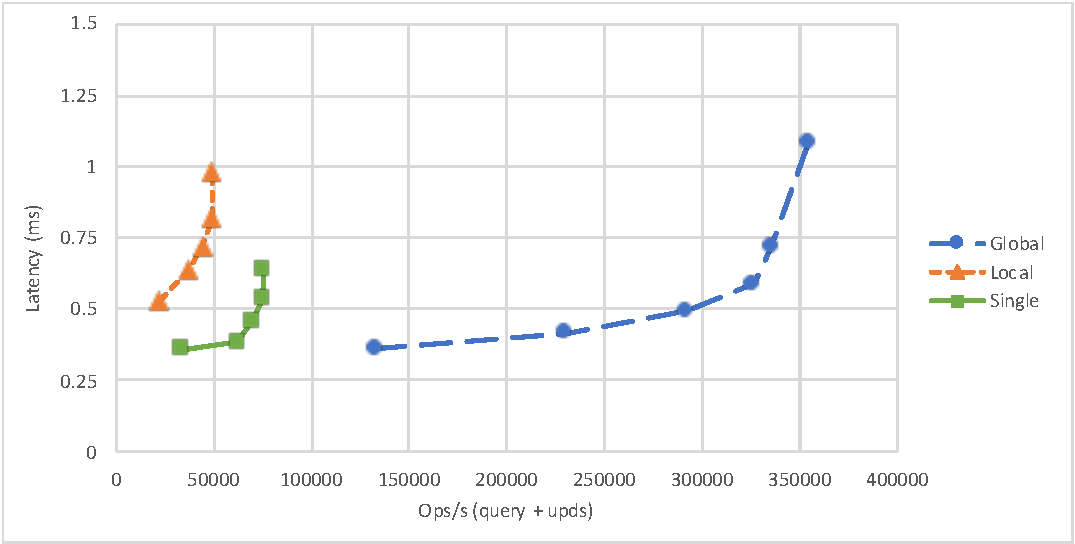
\includegraphics[width=.95\linewidth]{global_local_single_cut}
		\caption{All queries}
		\label{fig:global_local_single}
	\end{subfigure}%
	\begin{subfigure}{.5\linewidth}
		\centering
		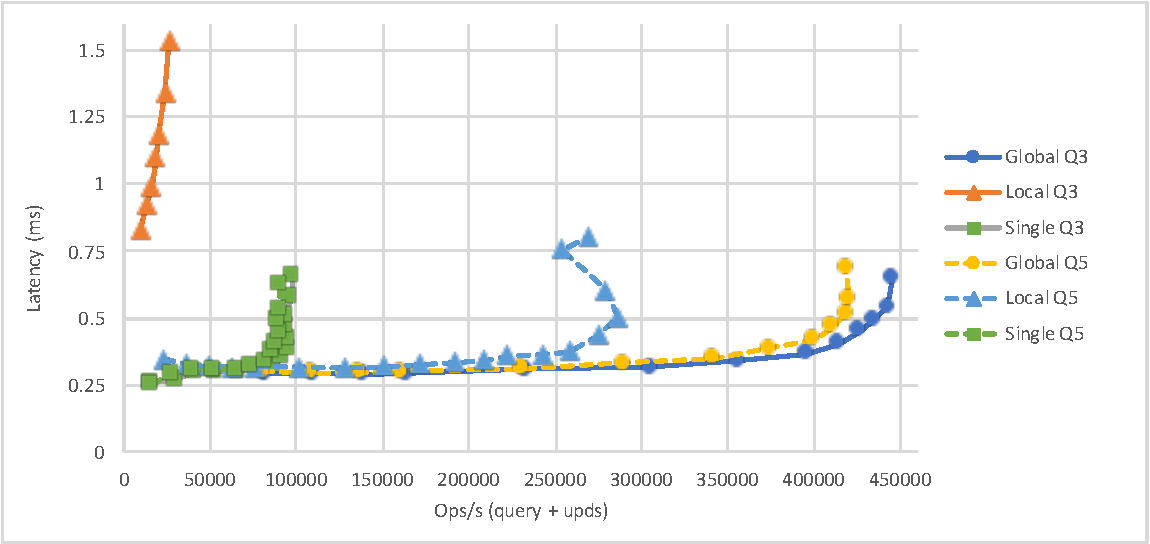
\includegraphics[width=.95\linewidth]{individual_query_cut}
		\caption{Single query type}
		\label{fig:q3q5}
	\end{subfigure}
	\caption{Query-only performance of PotionDB and its local and single index versions. On the left all queries are executed, while on right it is only Q3 or Q5.}
	\label{fig:query_only}
\end{figure}

Figure \ref{fig:query_only} shows the results of experiments for the three versions of PotionDB, in terms of query/s versus latency.
Figure \ref{fig:global_local_single} includes all queries in the execution, while \ref{fig:q3q5} only includes a single type of query at a time.

As expected, on both cases the performance of the local and single versions is worse than normal PotionDB.
Focusing on figure \ref{fig:global_local_single}, it is noticeable that local version performance is about 7 times lower than normal.
This happens because most queries require data from all regions, thus requiring local clients to contact all servers and wait for them all to reply.
This leads to both more load on each server as well as more time waiting on the client side.
The single scenario performance is roughly 1/5 of normal's.
This can be explained as all queries only need to consult the indexes, which due to those being all in one server, implies that the load is all directed to one server instead of being split across five.

Figure \ref{fig:q3q5} shows that the lower throughput of the local version is due to the locality of the data - Q3 requires data from all servers and has about 1/12 of the performance of normal PotionDB, while Q5 only requires data from one region (thus one server) and has about 2/3 of the performance.
This smaller drop can be explained due to local clients not being sticky - as the query parameters are selected at random, local clients are forced to constantly query different servers, while each normal client can query always the same server.

\subsubsection{PotionDB scaling - queries VS updates}

We now evaluate the impact on PotionDB's throughput of executing updates alongside queries, with multiple read/write ratios (\ref{enum:question2}).
In this scenario, whenever a client wants to execute an operation, it picks at random whenever a query or an update is executed.
It is worth noting that an update affects both base data and all associated indexes.
Also note that while index updates are executed in every replica, we only count them once (i.e., if one update is executed 5 times, it still only counts as 1 operation).

\begin{figure}
	\centering
	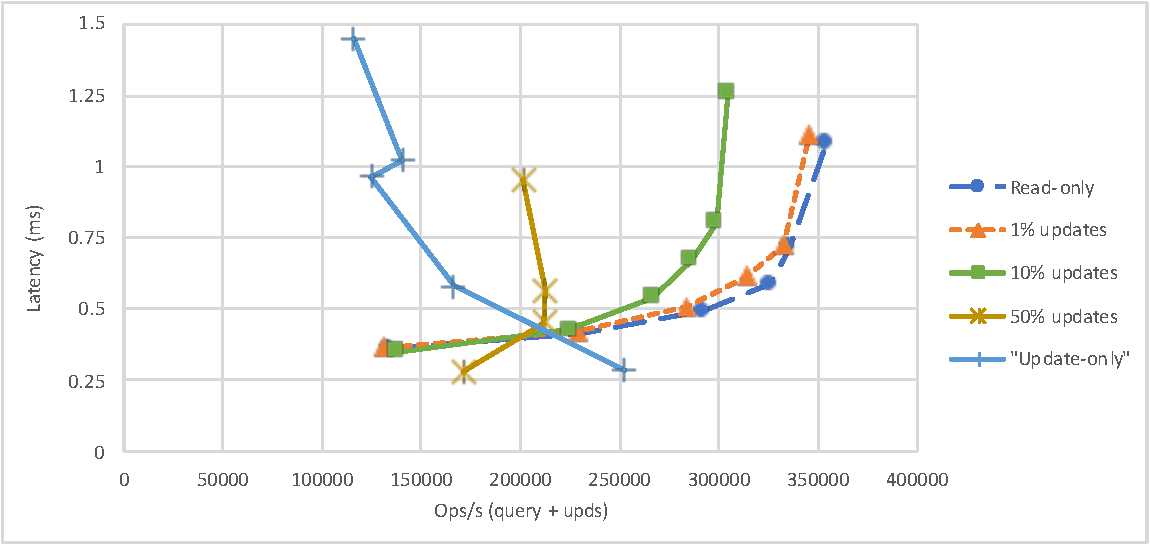
\includegraphics[width=.95\linewidth]{update_rates_cut}
	\caption{PotionDB performance with varying update rate.}
	\label{fig:update_rates}
\end{figure}
\begin{figure}
	\centering
	\begin{subfigure}{.5\linewidth}
		\centering
		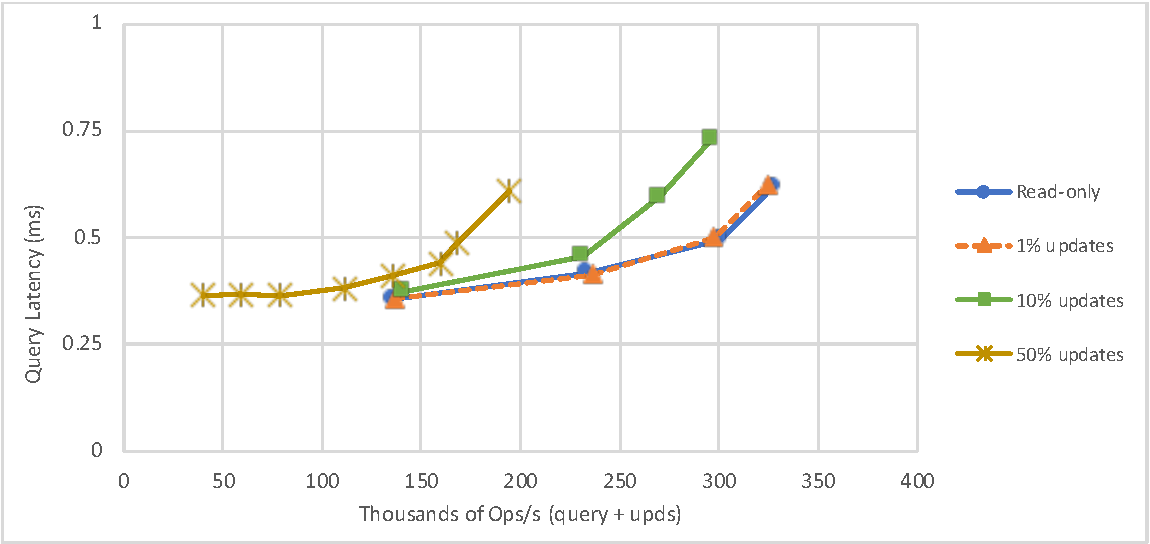
\includegraphics[width=.95\linewidth]{update_rates_query_cut}
		\caption{Query-latency}
		\label{fig:update_rates_query}
	\end{subfigure}%
	\begin{subfigure}{.5\linewidth}
		\centering
		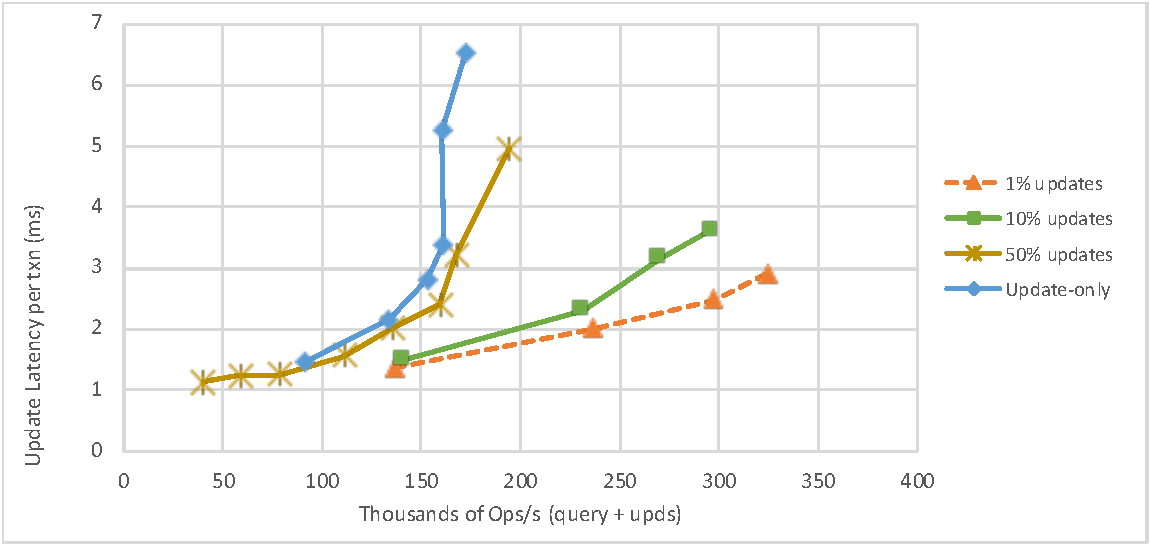
\includegraphics[width=.95\linewidth]{update_rates_update_cut}
		\caption{Update-latency}
		\label{fig:update_rates_update}
	\end{subfigure}
	\caption{PotionDB performance with varying update rate, with query and update latencies split. Note that updates are done in groups due to having to update both base data and indexes.}
	\label{fig:update_rates_split}
\end{figure}

Figure \ref{fig:update_rates} shows the results of executing updates alongside queries, with varying odds of choosing an update.
For low update rates (1\% and 10\%), the decrease in performance can be considered reasonable (aproximately 2,5\% and 14\%).
For higher rates, two observations can be made:
\begin{enumerate*}[label=(\roman*)]
	\item the servers saturate earlier, in some cases even decreasing throughput as the number of clients rises;
	\item the max throughput is lower.
\end{enumerate*}

The referred observations can be explained if we consider the following. 
With PotionDB's internal partitioning, queries on different objects can be executed concurrently, thus query-only scenarios scale easily. 
However, updates in a transaction must lock the partitions they're involved and do a 2-phase commit, in order to ensure the states evolve sequentially in a replica even when concurrent transactions are issued.
As such, if the update rate is high, clients executing queries or updates may often have to wait for a transaction with updates to finish executing before executing their own operations.
\andre{I might have to reffer in an early section with more detail how we do updates in our experiment, namely that our granularity is at order-level and that indexes, orders and items are updated in the same txn.}.

Figure \ref{fig:update_rates_split} shows the same experiment as figure \ref{fig:update_rates}, but showcases the latencies of queries and updates splitted, instead of together.
It is noticeable that updates have quite higher latencies and scale much less, which is due to both 2-phase commit and grouping of operations (as updates need to be reflected on both base data and indexes).


\andre{Probably some concluding note that reffers that for PotionDB's intented usages it is likely that updates are much less frequent than queries, or maybe even that updates could maybe be delayed?}

\subsubsection{Batching}

On the previous scenarios, each client only requested one query at a time, even through updates were executed in groups (whenever one update to a base object is usued, all associated indexes are updated in the same transaction).
With this we've noticed that, with a low number of clients, an update-only scenario actually has better throughput than a query-only scenario.
Thus, we now evaluate the effect observable on PotionDB's throughput if multiple queries are included in the same transaction (\ref{enum:question3}).

%\begin{figure}
%	\centering
%	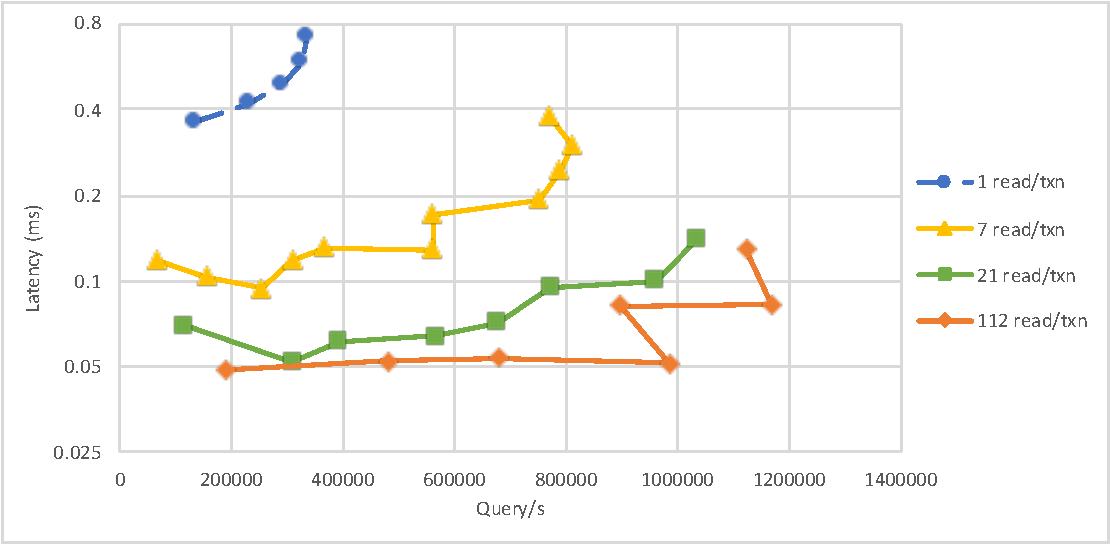
\includegraphics[width=.95\linewidth]{ops_per_txn_cut}
%	\caption{PotionDB performance when batching queries. Note that latency is in logarithmic scale.}
%	\label{fig:ops_per_txn}
%\end{figure}

\begin{figure}
	\centering
	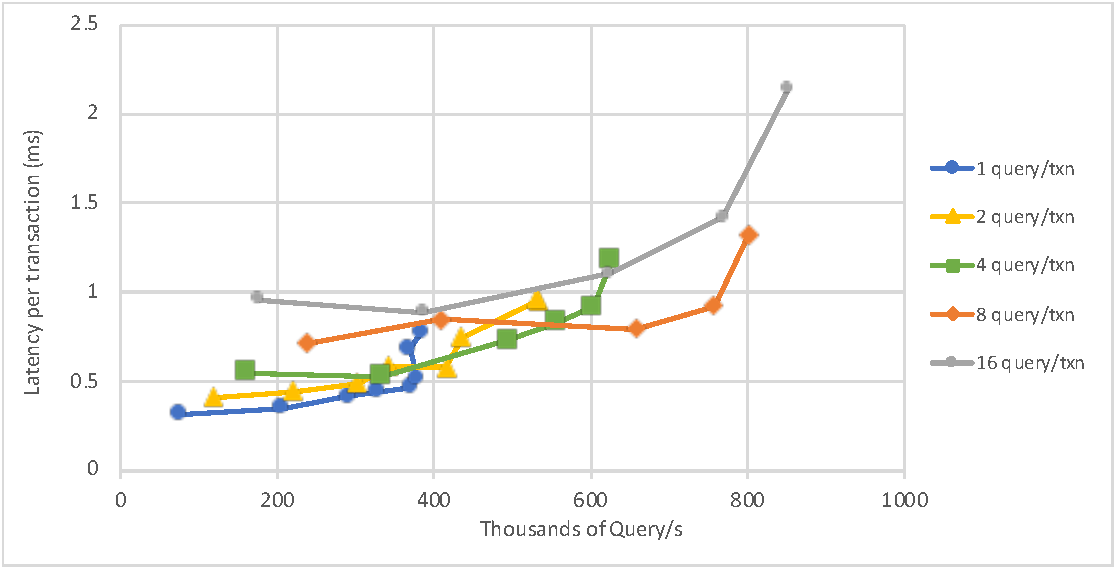
\includegraphics[width=.95\linewidth]{ops_per_txn_few_cut}
	\caption{PotionDB performance when batching queries. %Note that latency is in logarithmic scale.}
	}
	\label{fig:ops_per_txn}
\end{figure}

%\andre{Note: this graph is temporary - I'll have to repeat the tests with less clients and a few repetitions of the same executions. Also probably with lower values. When I first did this test it was more for curiosity than for really putting it here...}

Figure \ref{fig:ops_per_txn} shows how PotionDB scales in terms of query/s depending on how many queries are executed in each transaction.
As expected, as we increase the amount of queries per transaction, so does the latency, as there is more data to send, receive and process.
However, the beneficts for throughput are visible - comparing 1 query/txn with 8 query/txn, we can see the throughput more than double before the server saturates, and latency increase by less than double.
Increasing the number of queries/txn also leads to PotionDB saturating with less clients, as more time is spent on processing queries instead of waiting/switching clients, thus making better usage of machine resources.
%We can see that with batching PotionDB reaches its peak performance with a lower number of clients (high query/s with low latency), and is able to provide higher throughput with lower latency - up to 1.2M ops/s with batching compared to 0.36M ops/s without batching.

\subsubsection{CRDT Benchmark}

\andre{I didn't know what to title this}

We now evaluate how a single PotionDB server scales outside of the TPC-H scenario.
Namely we do a few benchmarks to determine the raw throughput of PotionDB when executing random operations, instead of specific queries or updates.

\begin{figure}
		\centering
	\begin{subfigure}{.535\linewidth}
		\centering
		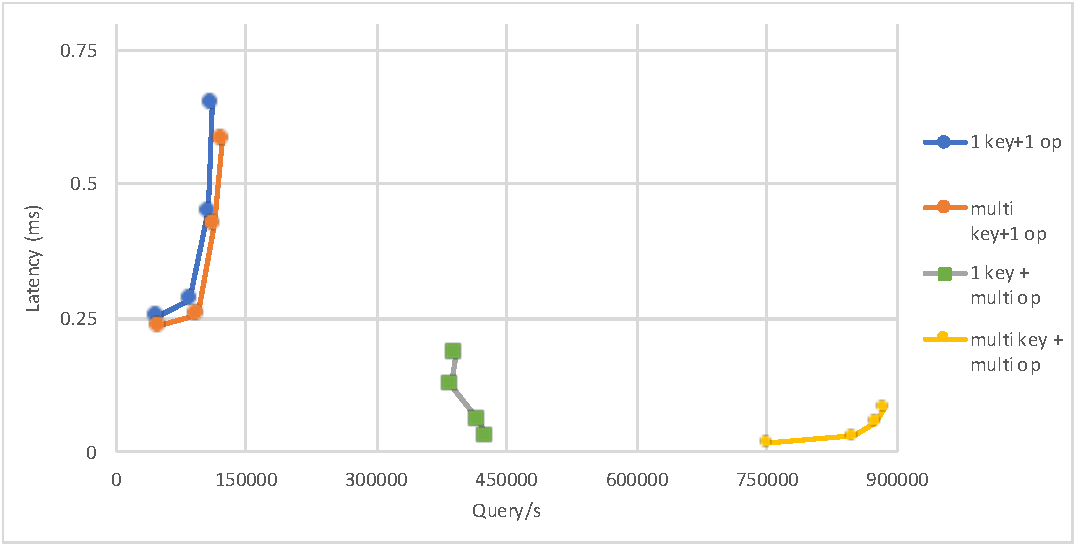
\includegraphics[width=.95\linewidth]{bench_read_cut}
		\caption{Read-only}
		\label{fig:bench_read}
	\end{subfigure}%
	\begin{subfigure}{.465\linewidth}
		\centering
		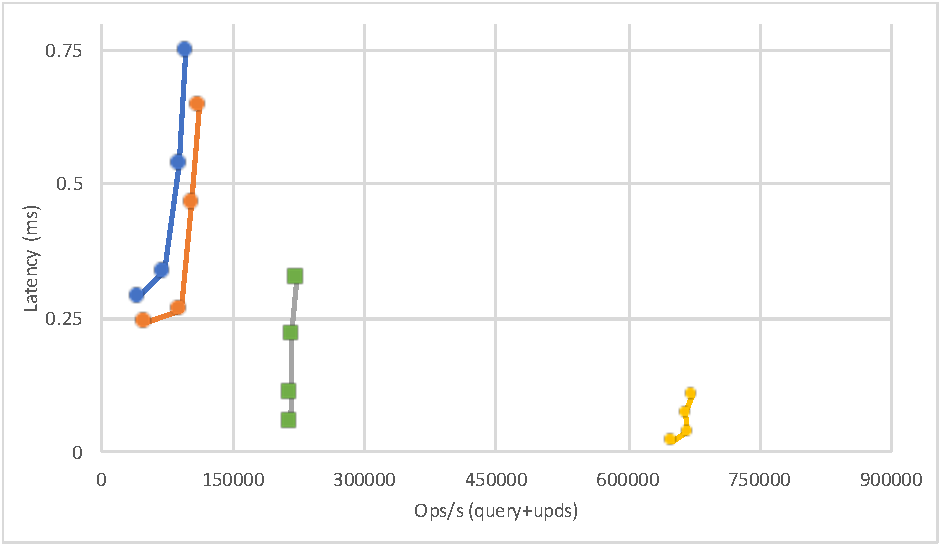
\includegraphics[width=.95\linewidth]{bench_update_cut}
		\caption{10\% update rate}
		\label{fig:bench_upd}
	\end{subfigure}
	\caption{Single server performance when executing random operations on set CRDTs. 1 key corresponds to a single CRDT shared between all clients, while multi key corresponds to multi CRDTs per client. 1/multi op refer to single or multi operation transactions.}
	\label{fig:bench}
\end{figure}

Figure \ref{fig:bench} contains results on the execution of benchmarks on set CRDTs.
Namely, figure \ref{fig:bench_read} concerns a read-only scenario, while \ref{fig:bench_upd} has a 10\% update rate.

Focusing on figure \ref{fig:bench_read}, it can be observed that increasing the number of operations per transaction greatly increases the throughput (up to 7x more in the tested scenario).
Increasing the number of CRDTs only seems to have a considerable effect when there's multiple operations in a transaction.
This may be due to the fact that a lookup operation in a set CRDT executes so quickly that most of the overhead may be in communication between threads or on converting data to the wire, thus not taking much benefict from the CRDTs being split across different partitions.

Considering figure \ref{fig:bench_upd}, considerably lower latencies can be observed when using multiple keys with only 1 operation per transaction.
Based on other tests we done, we can affirm that this difference is bigger the higher the rate of updates are.
This is due to the fact that updates must lock a partition, thus if different keys are used, and each client only manipulates one key at a time, some reads may be executed in parallel with updates, as long as it is for different partitions.
With a single key used by all clients, no concurrency is possible when an update is being executed.

The observed performance is worse than in a read-only scenario, 
which is specially noticeable in scenarios with multiple operations per transaction.
IThis is even more noticeable in the case with only one key, as the vast majority of transactions will include updates and thus the different clients end up having their transactions executed sequentially.
Having multiple keys eases this, as only partitions which get updated need to be locked, thus some concurrency is still possible.

\andre{This subsection VERY LIKELY needs to be rewritten/better thought of. Maybe even choose different data to show...}

%\subsection{Old Results}
%
%We first start by comparing the performance between running PotionDB in its intended mode, i.e., with views of global data, versus having each view only include data replicated locally.
%To distinguish between both, we call the former simply PotionDB and the later Local PotionDB.
%It is expectable for Local PotionDB to have worse performance, as most TPC-H queries concern data that is replicated across multiple replicas, which implies that clients need to contact multiple replicas to answer a single query in the case of local views.
%
%\begin{figure}
%	\centering
%	\begin{subfigure}{.5\linewidth}
%		\centering
%		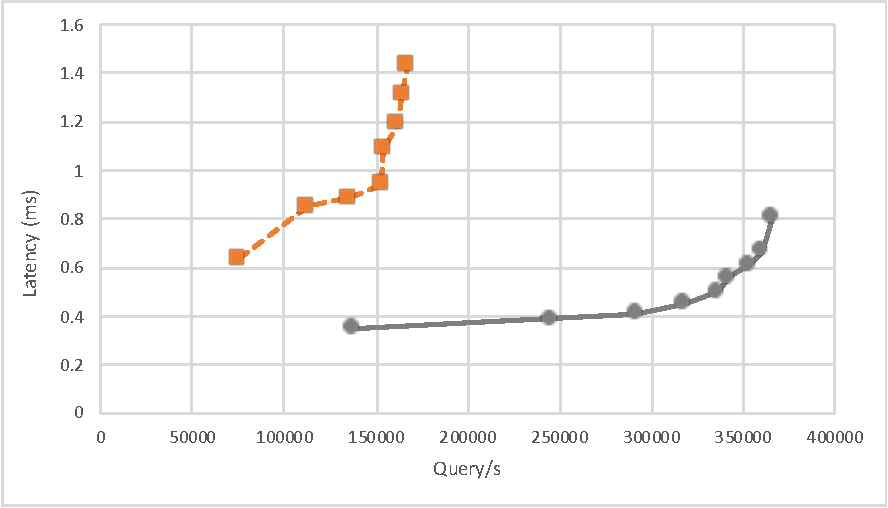
\includegraphics[width=.95\linewidth]{8_CPU_global_LQ_cut}
%		\caption{Global PotionDB}
%		\label{fig:global8CPU}
%	\end{subfigure}%
%	\begin{subfigure}{.5\linewidth}
%		\centering
%		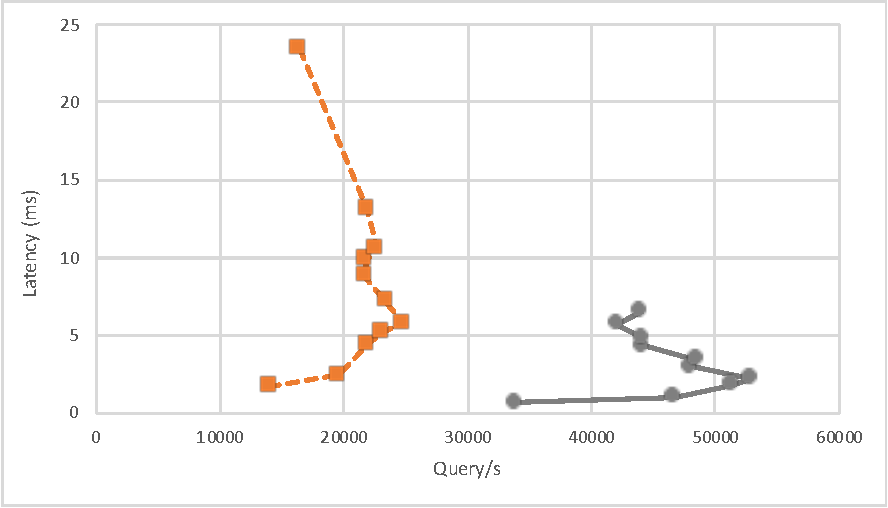
\includegraphics[width=.95\linewidth]{8_CPU_local_LQ_cut}
%		\caption{Local PotionDB}
%		\label{fig:local8CPU}
%	\end{subfigure}
%	\caption{Performance of PotionDB (left) with global indexes versus a version with local indexes (right). Square points represent the situation with both query clients and an update client, while circle is query only. Notice the difference in the scales between the graphs.}
%	\label{fig:8CPU}
%\end{figure}
%
%%\andre{Suggestions for graphs are more than welcome. Also, should instead of using Figure \ref{fig:global8CPU} and \ref{fig:local8CPU} use a single graph which contains both the local and global scenarios?}
%%
%%\begin{figure}
%%	\centering
%%	\begin{subfigure}{.5\linewidth}
%%		\centering
%%		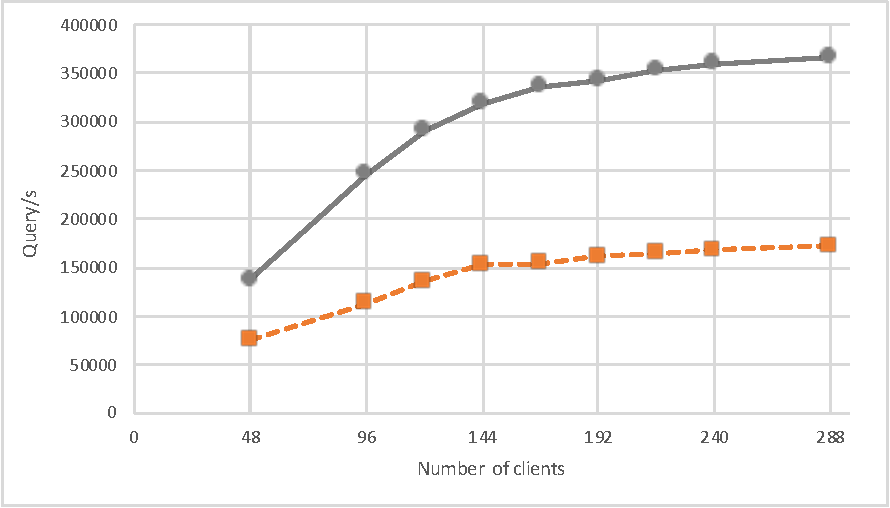
\includegraphics[width=.95\linewidth]{8_CPU_global_index_cut}
%%		\caption{Global PotionDB}
%%		\label{fig:global8CPU}
%%	\end{subfigure}%
%%	\begin{subfigure}{.5\linewidth}
%%		\centering
%%		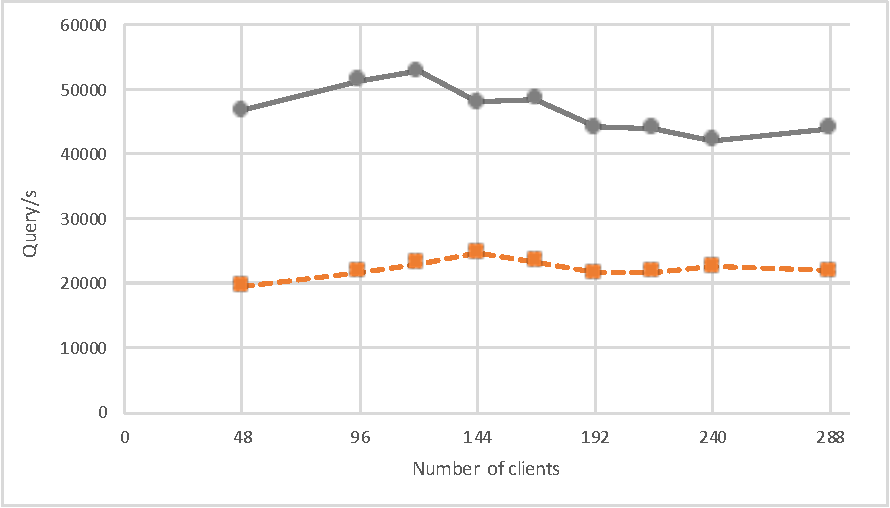
\includegraphics[width=.95\linewidth]{8_CPU_local_index_cut}
%%		\caption{Local PotionDB}
%%		\label{fig:local8CPU}
%%	\end{subfigure}
%%	\caption{Performance of PotionDB (left) with global indexes versus a version with local indexes (right). Square points represent the situation with both query clients and an update client, while circle is query only. Notice the difference in the y scale (query/s) between the graphs.}
%%	\label{fig:8CPU}
%%\end{figure}
%%
%
%\andre{TODO: Este texto é ainda o antigo!!!}
%
%Figure \ref{fig:global8CPU} and \ref{fig:local8CPU} show the results of experiments for, respectively, PotionDB and Local PotionDB in terms of query/s.
%There is at least two noteworthy points to be taken from the graphs.
%
%First, the number of queries that PotionDB can answer decreases to aproximately half when there are updates going on - this is expected, as due to causality PotionDB needs to ensure all reads of a transaction see the same version.
%This also implies that old object versions may need to be computed, which implies extra server work.
%
%Second, as expected, the local version has considerably lower performance than the global version, peaking its performance at a much lower number of clients (120 to be precise).
%In short this can be justified by considering that to answer a single query in the local version, multiple servers may need to be contacted. 
%To exemplify, consider the query "Top 10 product orders not yet shipped."
%This could be answered with a single Top-K CRDT read in the global scenario, but on the local scenario all servers need to be contacted as each server only knows of the orders done in its continent.
%Thus, the client has to wait for all servers to answer and then aggregate the results before moving to the next query.
%In other words, for some queries all servers need to reply to all clients and thus send/process more data, unlike with the global scenario in which each server is, in practice, dedicated to a subset of the clients.
%In conclusion, there is a performance gain to be obtained from having indexes of data replicated both locally and on other servers when there are queries that concern such data.


\section{Related Work}

Both strongly and weakly consistent solutions exist to support services that require geo replication of their data.
%Strong consistency solutions like Spanner \cite{???} \comment{likely introduce others}
%Some examples include, for strong, Spanner \cite{???} and ???; while for weak ??? and ???.
Strong consistency solutions like Spanner \cite{spanner} and CockroachDB \cite{cockroachdb} provide the ilusion of a single replica, thus making it easier to provide a consistent view for clients.
However, the CAP theorem \cite{cap} implies that availability may be compromised in case of network partitions, and high latency is expected as multiple datacenters need to be contacted for executing operations.
Weak consistent solutions such as Dynamo \cite{dynamo} and COPS \cite{cops} can provide highly available, low latency operations, but providing a consistent view of the database to clients is challenging.
Causal consistency is a sub-form of weak consistency that alleviates this problem, however anomalities can still be observed even with cross-object causality \cite{cops, burckhardt2013understanding}.

Systems like Dynamo \cite{dynamo}, COPS \cite{cops} and CockroachDB \cite{cockroachdb} provide geo-replication.
Dynamo provides partial replication, however reads and updates for multiple keys are done independently, thus there's no causal read of multiple reads.
COPS provides causal+ consistency and supports transactions for reads, however it doesn't support neither partial replication or views.
CockroachDB is strongly consistent and, thus, may fail due to network partitions, and does not provide partial replication.
 
CRDTs \cite{crdt} are replicated data types that guarantee state convergence, assuming all updates are eventually delivered.
Thus, they are often used in weakly consistent systems, e.g., Redis \cite{redisCRDT} and Riak \cite{riak}.
Some types of CRDTs have been introduced that can help with representing views of data, namely computational CRDTs \cite{computationalCrdt} and non-uniform CRDTs \cite{Cabrita17Nonuniform}.
The former computes some result over data (e.g., a sum), while the later focus on minimizing the information that needs to be replicated to correctly reply to queries (e.g.: a top-k CRDT doesn't need all entries to be replicated).
We leverage on both in our solution.

Alternative solutions to provide global queries on partially replicated data includes using distributed processing systems like Pixida \cite{kloudas2015pixida} or Hourglass \cite{hourglass}.
However, this impose challenges both consistency-wise, as well as in terms of latency and data transferred.
The amount of data to be transfered is specially concerning, as if the underlyng systems only provide simple get operations, very high amounts of data may have to be transfered to reply to a small query like a top 10.
PotionDB avoids this by having materialized views, which allows to have only the required data replicated in every server and thus reply to such query efficiently.
%COPS doesn't support partial replication
%Dynamo supports partial replication, but doesn't support views or consistent reads of multiple objects.
%Start talking about partial replication
%Mention some geo-distributed DBs, explain that they don't provide partial replication
%CRDTs, non-uniform replication
%Maybe at some point refers transactions
%Refer alternative solution of pixida/parallel jobs.
%Maybe mention views in consistent databases.
%Hourglass is mentioned in Pixida paper.



\section{Conclusions}

\bibliographystyle{abbrv}
\bibliography{bib}

\null\newpage\null

\null\newpage\null

\section{Topics}

This contains the topics that were initially discussed during the first meeting and some afterthoughts.

\section{System overview}

\begin{itemize}
	\item System model
	\begin{itemize}
		\item Replicação parcial
	\end{itemize}
	\item System API
	\begin{itemize}
		\item "Create table"
		\item "Create view"
		\begin{itemize}
			\item CRDT não uniforme
			\item put numa table $\implies$ puts nas várias views
			\begin{itemize}
				\item consistência das views face aos dados - in sync
			\end{itemize}
		\end{itemize}
	\end{itemize}
	\item System description
	\begin{itemize}
		\item CRDT não uniforme
		\item Implementação de queries?
	\end{itemize}
	
\end{itemize}

\section{Implementation}

\section{Evaluation}

%- Dizer o que se vai avaliar.
%- Ter um gráfico com o que seria de esperar.

\section{Related Work}

\section{Conclusions}

\section{System overview}
Possiveis pontos mais detalhados?

\subsection{System model}

\begin{itemize}
	\item Network assumptions
	\item Client-server interaction (refer key-value store interface? Maybe refer this instead in System API?)
	\item Server-server interaction? (is it needed? We'll already touch this in Replication.)
	\item System guarantees
	\begin{itemize}
		\item CRDTs
		\item Consistency level	
	\end{itemize}
	\item Replication
	\item Async
	\item Op-based
	\item Maintains consistency, i.e., transaction level based.
	\item Partial (system admin defined, each server only has a subset of the data based on topics. Potencially some data can be replicated everywhere)
\end{itemize}

\subsection{System API}

\begin{itemize}
	\item Basically how can we translate a problem to sql-like operations
	\item Create table
	\item Create view
	\item Updates (incluir problema de consistência de views/dados)
	\item Queries (incluir aqui problema de os CRDTs não uniformes precisarem de mais dados? Ou na zona da view?)
\end{itemize}

\subsection{System description}

\begin{itemize}
	\item Structure? Maybe that's for implementation? How much detail?
	\begin{itemize}
		\item Internal partitioning vs external partitioning? Capaz de não ser boa ideia...	
	\end{itemize}
	\item CRDTs and non-uniform CRDTs?
\end{itemize}

\andre{I ended up describing the topics of system description in other subsections, apart from Structure. I don't recall going into much detail of what a CRDT is, but that shouldn't be necessary anyway.}

\section{Implementation}

\begin{itemize}
	\item Go
	\item Transactions (TM/Mat?)
	\item Replication (RabbitMQ and other stuff?)
	\item Communication (protobufs. Also worth noticing the compability with existing AntidoteDB clients)
	\item CRDTs (version management at least)
\end{itemize}

\andre{A good part of the implementation is already included in other sections, at least indirectly. Mainly Replication and to an extent Transactions/Communication. We need to decide what really is important to refer in the "implementation" section.}

\end{document}
